%!TEX root = ../main.tex
\chapter{Enfermedad de Chagas}
\label{chap:chagas}

La enfermedad de Chagas es considerada como negligenciada por la \gls{oms} y es causada por el protozoo flagelado Trypanosoma Cruzi. Esta enfermedad es poco estudiada pese a que afecta a millones de personas, tiene una tasa muy alta de incidencia en países en vías de desarrollo y su tratamiento es  costoso~\cite{trouiller2002drug}. 

La enfermedad se puede observar desde México hasta Sudamérica, aunque se pueden presentar casos en Estado Unidos y Canadá. Las zonas rurales son las más afectada produciendo mas de 10.000 muertes al año~\cite{lozano2013global}. En etapas iniciales síntomas que presenta la enfermedad son fiebre, linfadenopatía, aumento del tamaño del hígado y bazo, miocarditis o meningoencefalitis. En casos crónicos se presentan los síntomas: cardiomiopatía, dilatación patológica del esófago y colon~\cite{nery1968surto}. 

El método de transmisión es por medio de las heces de insectos triatominos hematófagos. Los cuales habitan principalmente en las grietas de viviendas precariamente construidas en zonas rurales. La transmisión también puede darse por medio de transfusiones de sangre, trasplante de órganos y de madres infectadas a los hijos durante el embarazo, pero estos casos son mas raros.

El parásito Trypanosoma cruzi, tiene un ciclo biológico complejo, su morfología y expresión antigénica cambia de acuerdo al lugar donde se encuentra. El parásito presenta tres tipos morfológicos funcionales: epimastigotes, tripomastigotes y amastigotes como se muestra en la Figura \ref{img:imagen-amastigotes1}. El tipo morfológico que estudiaremos es el amastigote en el cual el flagelo esta reducido o ausente.

\begin{figure}[h!]
\centering
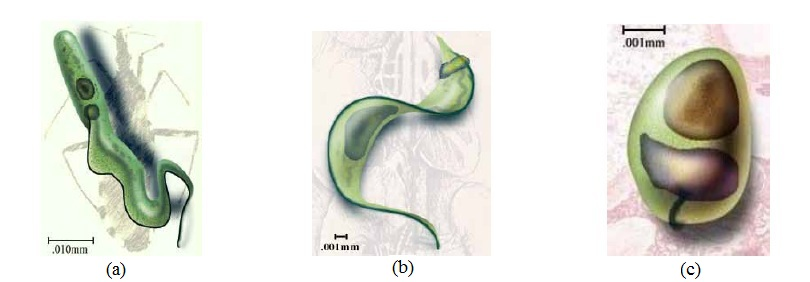
\includegraphics[width=90mm]{./figuras/amastigotes1.jpg}
\caption{(a) Epimastigotes. (b) Tripomastigotes. (c) Amastigotes}
\label{img:imagen-amastigotes1}
\end{figure}

El primer paso para determinar la eficacia de nuevos fármacos antichagasicos y así reducir el costo del tratamiento es el recuento de la forma parasitaria intracelular(amastigote) al microscopio~\cite{de2006analise}. 

En el contexto del tratamiento de las imágenes de amastigotes intracelulares de Trypanosoma Cruzi se citan trabajos que segmentan las imágenes a partir de la adquisición automatizada de imágenes de fluorescencia~\cite{engel2010image}~\cite{nohara2010high}. Las técnicas anteriores son específicas para el tipo de imágenes a la cual fueron aplicadas y es necesaria la adaptación de las mismas para cada tipo celular.

\begin{figure}[h!]
\centering
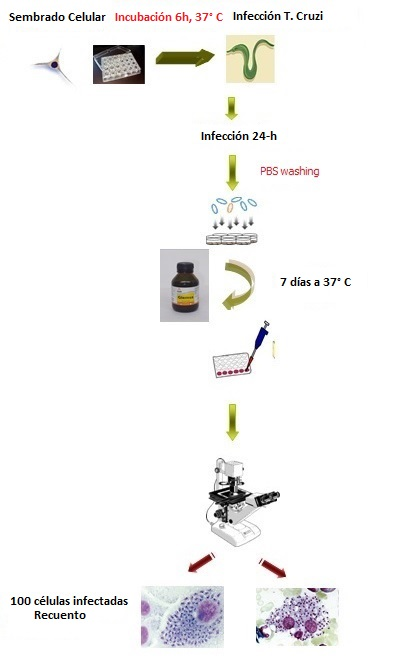
\includegraphics[width=90mm]{./figuras/amastigotes2.jpg}
\caption{Recuento de amastigotes vistos en el microscopio electrónico}
\label{img:imagen-amastigotes2}
\end{figure}

Como se muestra en la Figura \ref{img:imagen-amastigotes2} para realizar el conteo de forma manual de la cantidad de amastigotes presentes en las células infectadas las mismas son teñidas con el colorante Giemsa. Los núcleos y los amastigotes son teñidos de un color azul oscuro lo que permite que sean visualizadas y distinguidas al microscopio con un aumento de 1000x. Con el objetivo de disminuir los errores del investigador debido a la subjetividad de la técnica, el recuento se realiza por triplicado y se promedian los resultados~\cite{mendez1996leishmania}.

Para realizar el conteo de forma automática se puede utilizar la transformada de watershed con marcadores internos y externos como técnica de segmentación y la etiquetación de componentes conectados para el conteo. Este proceso ya se ha realizado en imágenes en escala de grises y demuestra ser eficiente y tener una baja tasa de error~\cite{noguera2013mathematical}. El trabajo presentado por Vázquez et al. solo se ha realizado en imágenes en escala de grises, esto deja abierta la posibilidad de mejorar la segmentación al obtener mayor información mediante el uso de imágenes a color.

\section{Resumen}

En este capítulo se presentaron los conceptos mas relevantes de la enfermedad de chagas, considerada como negligenciada por la \gls{oms}, el cual es producido por el parásito Trypanosoma cruzi. El parásito puede tener varias formas y la que estudiaremos se denomina amastigote. La segmentación de los componentes en imágenes celulares es importante para realizar el conteo de los amastigotes y así determinar la eficacia de los fármacos antichagasicos.